\documentclass[12pt, a4paper, lithuanian, final]{article}

\usepackage{hyperref}
\usepackage{graphicx}
\usepackage{float}
\usepackage{placeins}
\usepackage{gensymb}
\usepackage{xcolor}
\usepackage{listings}
\usepackage{amsmath}
\usepackage{textgreek}
\usepackage{mathtools}
\usepackage[obeyFinal]{easy-todo}
\usepackage[utf8]{inputenc}
\def\LTfontencoding{L7x}
\usepackage[\LTfontencoding]{fontenc}
\usepackage[lithuanian]{babel}
%\usepackage{times}

%\renewcommand{\sfdefault}{uhv}
%\renewcommand{\rmdefault}{utm}
%\renewcommand{\ttdefault}{ucr}

\usepackage{VUMIF}

%Kodo highlitinimo configas
\lstset{basicstyle=\ttfamily,
	showstringspaces=false,
	commentstyle=\color{red},
	keywordstyle=\color{blue}
	}


% Titulinio puslapio reikalai
\vumifdept{Programų sistemų katedra}
\vumifpaper{}
\title{Praktikos uždarojoje akcinėje bendrovėje "`Elektromotus"' ataskaita}
\author{
    4 kurso 1 grupės studentas \\
    Rytis Karpuška
}

\supervisor{Irus Grinis, doc.}
\date{Vilnius \\
	2014}


\begin{document}

%titulinis ir turinys
\maketitle

\vumifsectionnonum{Įvadas}


%Skyrius apie įmonę
\section{Apie UAB "`Elektromotus"'}

UAB "`Elektromotus"' 2010 metais įkurta trijų steigėjų: Gintauto Palucko, Mindaugo Milašausko ir Šarūno Šutavičiaus su tikslu realizuoti jų sukauptą patirtį elektromobilių valdymo sistemų kūrimo srityje.
Nuo to laiko, įmonė išaugo ir samdyti darbuotojai pilnai perėmė įmonės darbo krūvius.
Šiuo metu įmonėje yra per 15 darbuotojų, metinė apyvarta viršyja milijoną litų, bei vykdomas ne vienas naujas projektas, su tikslu, patobulinti, išleisti, sukurti naujas technologijas bei produktus.

Buvo sukurti ir išleisti keli produktai, bei patentai.


\subsection{Produktai}
\subsubsection{"`Emus BMS"' - Baterijų valdymo sistema}
"`Emus BMS"' yra pagrindinis ir seniausias įmonės produktas, įnešantis daugiausiai pajamų.

Tai yra valdymo sistema vidutinėms ir didelėms ličio jonų, ličio polimerų, ličio geležies fosfatų, nikelio-metalo hidratų ir kitoms baterijoms.

Sistemą sudaro trijų lygmenų hierarchinė struktūra:

\begin{figure}[H]
\begin{center}
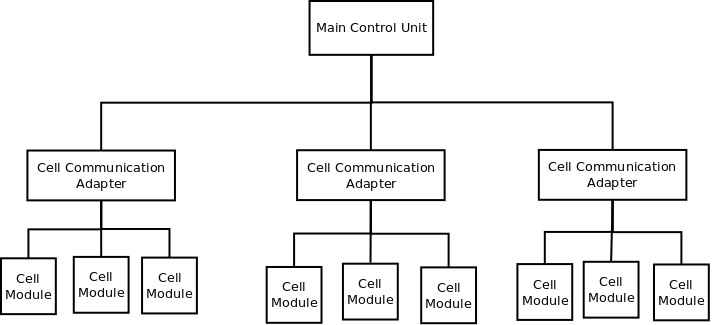
\includegraphics[width=1\textwidth]{img/bms_desc.png}
\caption{Emus BMS struktūra.}
\end{center}
\end{figure}

Sistemą sudaro šie komponentai:
\begin{itemize}
	\item{Main Control Unit} - Pagrindinis valdymo blokas, komunikuoja su komunikacijos adapteriais CAN sąsaja.
	\item{Cell Communication adapter} - Adapteris persiunčiantis CAN sąsajos komandas į celių modulius privačia įmonės sukurta sąsaja pritaikyta dirbti EMI triukšmingose sąlygose.
	\item{Cell module} - Celių moduliai, galiniai įrenginiai, matuoja celės įtampą, temperatūra, turi šiluminio balansavimo palaikymą.
\end{itemize}

Panašių sistemų rinkoje labai mažai, tad šį susilaukė populiarumo.
Ši sistema yra naudojama įvairiuose elektromobiliuose, laivuose, kranuose. ir t.t.

Ryškiausi klientų pasiekimai su "`Emus BMS"':
\begin{itemize}
	\item Komandos "`ACCIONA"' bolidas dalyvavęs "`Dakar"' ralyje
	\item Academic Motorsports Club Zurich (AMZ) automobilis, pasiekęs 100km/h per 1.785s, taip sumušdamas pasaulio rekordą
	\item "`Intersolar 2013, Munich"' saulės jegainės valdikliuose
	\item "`EcoPower Hybrid"' kranas dirbantis texaso uoste
	\item "`Lloyds paxter"' Pašto elektromobiliuose norvegijoje
\end{itemize}











%Skyrius apie mano veiklą įmonėje
\section{Veikla praktikos metu}

Praktikos metu įmonėje dirbau prie naujo įmonės projekto.
Projekto metu buvo sukurta sistema skirta geležinkelių aukštos įtampos kabelio vibracijoms tirti.
Sistema seka Šeimininko-Vergo (eng.: Master-Slave) topologiją, leidžiančią vienu metu palaikyti iki 16 "`Slave"' tinklo mazgų.

\begin{figure}[H]
\begin{center}
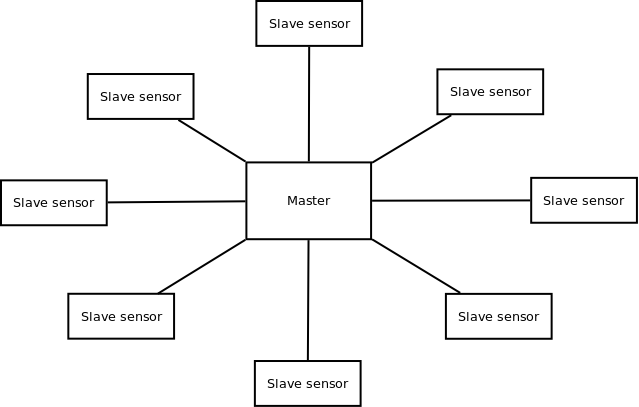
\includegraphics[width=1\textwidth]{img/NorgeRail_star.png}
\caption{Vibracijų sensorių tinklo topologija.}
\end{center}
\end{figure}

Šio projekto metu buvo sukurti mazgų planavimo (eng.: scheduling), paketavimo, ir kiti algoritmai pritaikyti labai žemam elektros suvartojimui.
Ramiom darbo sąlygom techninė radio ryšio įranga dirba mažiau nei 1\% laiko.
Tai leido "`Slave"' sensoriams be pertraukimų atlikti matavimus nenutrūkstamai iki 7 dienų iki baterijos išsikrovimo.

Negana labai aukštų reikalavimų elektros suvartojimui, šie sensoriai turi stabiliai dirbti labai EMI triukšmingoje aplinkoje, nes jie montuojami teisiogiai ant aukštos įtampos kabelio.
Tam buvo sukurta speciali dėžutė imituojanti faradėjaus narvo savybes.

%TODO: Internet access

\subsection{Naujos Testavimo procedūros}

Prasidėjus profesinei praktikai projektas jau buvo pažengęs ir buvo atlikti bandymai realiuose geležinkeliuose su realiais traukiniais Trondheim ir Oslo traukinių stotyse, Norvegijoje.
Deja, praktika parodė, kad sistemoje buvo nemažai defektų, tame tarpe ir kritinių, dėl kurių buvo įmanoma pilnai prarasti ryšį su "`Slave"' sensoriais.
Todėl buvo nuspręsta, kad reikia sustiprinti testavimo procedūras.

\subsubsection{"`Checker"' modulis}

Įterptinės sistemos daugeliu atveju pasižymi palyginus silpnais procesoriais, kilobaitų eilės "`RAM"', "`FLASH"' atmintimis, bei labai limituotom derinimo sąsajom.
Dažna situacija kuomet vienintelis kelias derinimui yra "`JTAG"' ar panašaus tipo derintuvai, ar paprastesniais atvejais "`UART"' sąsaja su kompiuteriu, galinti išspausdinti tekstinę informaciją.
Tai buvo mūsų situacija.
Deja derinimas su tokiais įrankiais yra labai sudėtingas, ypač kai aplikacija yra realaus laiko ir labai jautri nenumatytiems uždelsimams.
Taip yra dėl to, kad pats derinimo veiksmas reikalauja uždelsimų, kurie iškreipia normalų programos darbą, o 10 mikrosekundžių užgaištos spausdinant vieną raidę, gali lemti programos darbo sutrikimus.

\paragraph{Sprendimo įdėja}
Kol "`UART"' sąsaja yra labai lėta, tai atminties operacijos šiuose procesoriuose yra ypatingai greitos dėl jų SRAM technologijų.
Atminties priėjimas užtrunka vos keletą ciklų.

%TODO continue here about solution and "checker" module








\subsubsection{Regresiniai vienetų testai}








%Ko pasiekiau per tą laiką
\section{Rezultatai}


\subsection{Vidutinis klaidų paieškos laikas}

\subsection{Sugauti defektai regresinio vienetų testavimo metu}



\section{Išvados}

\bibliography{Bibliografija}
\begin{itemize}
	\item [[SM04]] - \textit{Taming the Embedded Tiger – Agile Test Techniques for Embedded Software}, \url{http://www.leanagilepartners.com/library/XR5_Taming_Embedded_Tiger.pdf}

\end{itemize}





\end{document}



